\section{Definition of Knitting Pattern and Knitting Pattern Chart}

A knitting pattern specifies a set of instructions outlining the steps necessary to create a knitted textile or fabric. For knitting a fabric the knitter uses two or more knitting needles and a long, continuous strand of yarn which they use to form intersecting loops with, which in turn creates a textile or fabric. ``Knitting is a conversion system in which yarn loops are interwoven to form a fabric'' (\cite[p17]{Raz1993}). The type of loops the knitter uses as well as the kind of yarn determine the attributes of the knitted piece: elasticity, form and texture. A knitted fabric can be stretched in both horizontal and vertical directions, as well as the directions in-between. This makes it stand apart from woven fabric, which is created by layering two threads in an interlaced manner. The woven cloth is generally limited in its ability to stretch and be formed.

Knitting patterns can come in form of written instructions, usually with abbreviations used for the stitch terms, e.g. k2tog for the ``knit two together'' stitch, or in form of a pattern chart which consists of a grid filled with symbols. Both written patterns and pattern charts, are generally split into rows, where each row has a finite number of stitches. Each cell in such a grid signifies a stitch in the pattern and the symbol displayed in a cell corresponds with the stitch that needs to be made in that place in the pattern. In what order the rows have to be knitted depends on the chart type; some charts display only the uneven numbered rows, which belong to the \gls{RS} of the knitted fabric, and expect the knitter to knit the return row on the \gls{WS} inverse to the \gls{RS}, i.e. knits would be knitted as purls and purls as knits. Other charts show all rows, the uneven numbered for the \gls{RS} and the even numbered ones for the WS.

So far there does not exist an international standard for the symbols used in knitting charts or the abbreviations in written instructions. Symbols used by the industry usually vary depending on the region (\cite[p57]{Raz1993}) and it is the norm that a knitting pattern includes a glossary for the symbols and abbreviations used in the pattern. One exception to this is Japan, where there exists a Japanese Industrial Standard on knitting symbols used in the industry and for the hobby hand knitters: JIS L 0201-1995 (\cite{JKCA1995}). This leads to Japanese knitting pattern charts being published without a glossary of the symbols used.

Other regional industry standards that Raz mentions in his book are the German Standard and the needle notation system, ``the most explicit and accurate of all  notation systems'' (\cite[p58]{Raz1993}), which is solely used for industrial knitting machines and shows the positions of the needles of the knitting machine for each stitch.

\section{Comparison of Existing Solutions}

\subsection{Android apps}
When searching for the term ``knitting'' in the Google Play Store, Android’s official source for Google-approved applications, few results pop up. Next to a surprising amount of games about knitting, there are apps for knitting counters, knitting patterns and knitting instructions for those who wish to begin knitting. The following sections will look at the top five apps for creating and managing knitting projects with row counters and pattern display, as well as knitting chart creation.

\addcontentsline{toc}{subsubsection}{knit tink | Row Counter by Jennifer K. Warren}
\subsubsection*{knit tink | Row Counter by Jennifer K. Warren}

\textit{ The app can be found at \url{https://play.google.com/store/apps/details?id=com.warrencollective.knittink} \small{(last accessed: 2016-08-11)}}
\vspace*{0.5cm}

\noindent Out of all most popular knitting apps, knit tink features the most modern and clean design. The app can be used for free or bought as an ad-free pro version. Features include the creation, editing, viewing, and deletion of projects, the setup of one row, and one repeat counter per project, as well as the unlinking of the row counter from the repeat counter. The free version of the app restricts the number of projects to three. The developer announced an on-screen display of a knitting chart in PDF format as an upcoming feature.

\begin{figure}[H]
  \centering
    \begin{subfigure}[b]{0.4\textwidth}
      \centering
        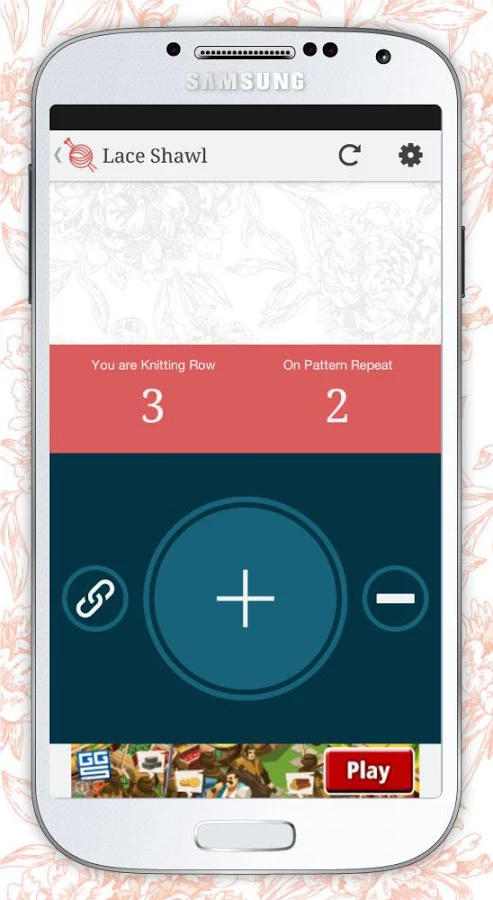
\includegraphics[width=0.95\linewidth]{images/image10.png}
        \caption[Row counter \protect{\small at: \url{https://lh6.ggpht.com/-9DvA3pUKqPQwDwi8P_mZXOEhyKz9pE4Dks2QuEKxEGJePvXfY4hUkLO0i-zud38c5Y=h900-rw} (last accessed: 2016-04-04)}]{Row counter}
      \label{fig:knit_tink_row_counter}
    \end{subfigure}
    \begin{subfigure}[b]{0.4\textwidth}
      \centering
        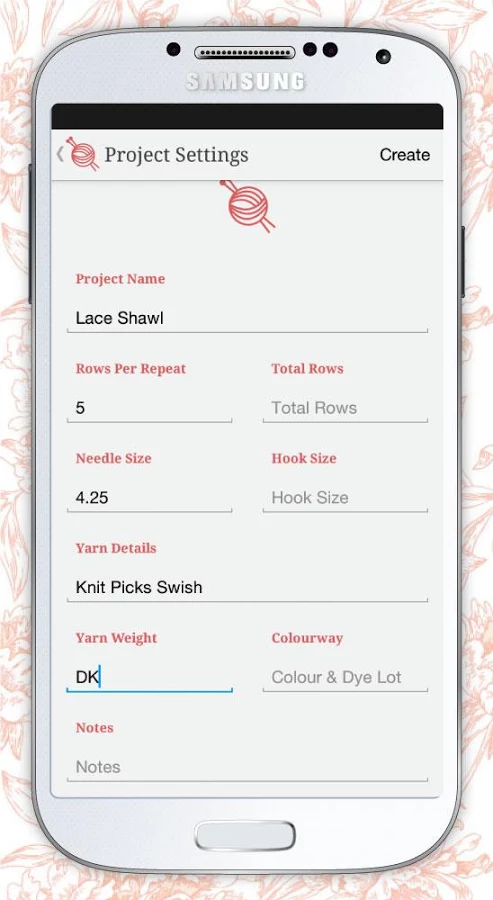
\includegraphics[width=0.95\linewidth]{images/image11.png}
        \caption[
            Project setup \protect{\small from: \protect\cite{knittink_project_setup}}
        ]{Project setup from \protect\cite{knittink_project_setup}}
      \label{fig:knit_tink_project_setup}
    \end{subfigure}
  \caption[Screenshots of the app knit tink \protect{\small at: \url{https://play.google.com/store/apps/details?id=com.warrencollective.knittink} (last accessed: 2016-08-08)}]{Screenshots of the app knit tink}
\end{figure}

\addcontentsline{toc}{subsubsection}{Knitting Counter by mkacki}
\subsubsection*{Knitting Counter by mkacki}

\textit{ The app can be found at \url{https://play.google.com/store/apps/details?id=org.kuklake.rowCounter} \small{(last accessed: 2016-08-11)}}
\vspace*{0.5cm}

\noindent Knitting Counter offers the same features as the knit tink app, the only differences being the layout of the user interface and the option to keep the phone from going into sleep mode, i.e., turning the phone screen off.

\begin{figure}[H]
  \centering
    \begin{subfigure}[b]{0.33\textwidth}
      \centering
        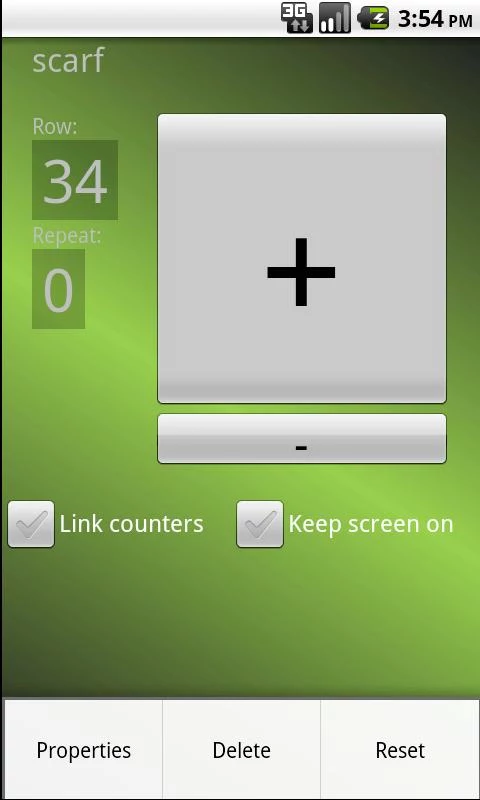
\includegraphics[width=0.95\linewidth]{images/image12.png}
        \caption[Row counter \protect{\small at: \url{https://lh4.ggpht.com/M05RYCkE7md51ckjB9Bf_CQjz-L6fSS3aWFnQ8UAoURXjO4BuHZiWeHtImzAhhpvekE=h900-rw} (last accessed: 2016-04-04)}]{Row counter}
    \end{subfigure}
    \begin{subfigure}[b]{0.33\textwidth}
      \centering
        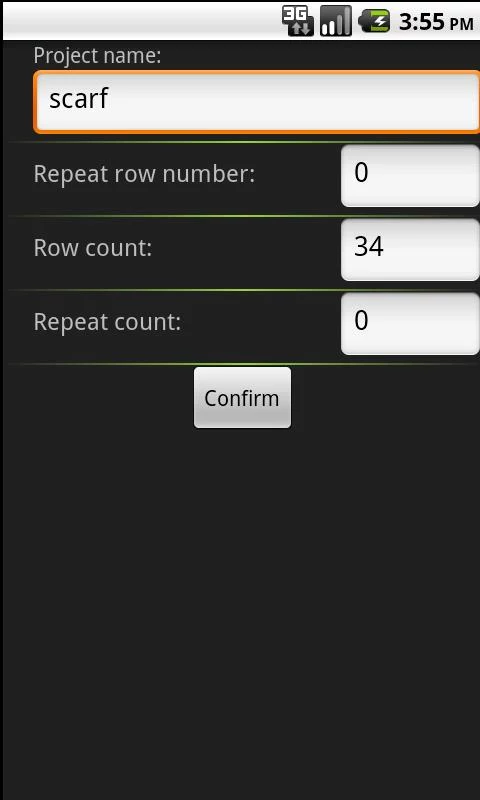
\includegraphics[width=0.95\linewidth]{images/image06.png}
        \caption[Row counter setup \protect{\small at: \url{https://lh3.ggpht.com/AuzeRh7n_r4yLpk9puanH0pBDhcxj6AwC8h5qCaMN3TsRMRu7rML9awuPZTf49M_ejo=h900-rw} (last accessed: 2016-04-04)}]{Row counter setup}
    \end{subfigure}
  \caption[Screenshots of the app Knitting Counter \protect{\small at: \url{https://play.google.com/store/apps/details?id=org.kuklake.rowCounter} (last accessed: 2016-08-08)}]{Screenshots of the app Knitting Counter}
\end{figure}

\addcontentsline{toc}{subsubsection}{Knitting and Crochet Buddy by Colorwork Apps}
\subsubsection*{Knitting and Crochet Buddy by Colorwork Apps}

\textit{ The app can be found at \url{https://play.google.com/store/apps/details?id=androiddeveloperjoe.knittingbuddy} \small{(last accessed: 2016-08-11)}}
\vspace*{0.5cm}

\noindent The Knitting and Crochet Buddy contains a plethora of features related to knitting and crocheting. As is the standard with the previously mentioned apps, it offers the possibility to manage different knitting and crocheting projects, with each a row and a repeat counter per project. Users can also enter written instructions or add a picture of the pattern chart to be displayed on the counter screen.

Additional features include: yarn and crochet symbol charts, an abbreviation chart, size charts for knitting needles and crocheting hooks, a project timer, a ruler function, and a flashlight.

\begin{figure}[H]
  \centering
    \begin{subfigure}[b]{0.5\textwidth}
      \centering
        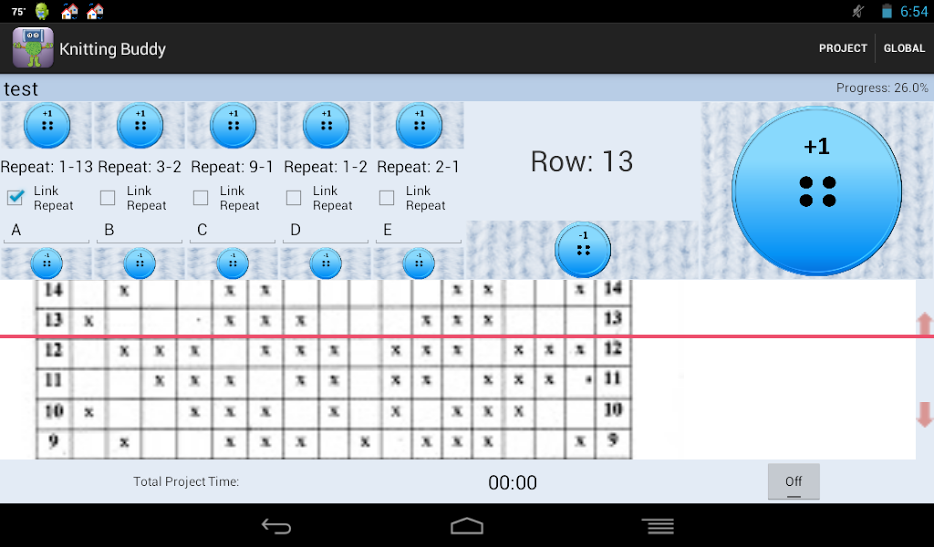
\includegraphics[width=0.95\linewidth]{images/image04.png}
        \caption[Row counter with pattern chart picture \protect{\small at: \url{https://lh3.ggpht.com/KJfgkhsUvqPCJSxqd7TfO9gVRgivtng8nfHgUENAHx401J-EqgPvTbCMW-dTrWVqzJE=h900-rw} (last accessed: 2016-04-04)}]{Row counter with pattern chart picture}
    \end{subfigure}
    \begin{subfigure}[b]{0.33\textwidth}
      \centering
        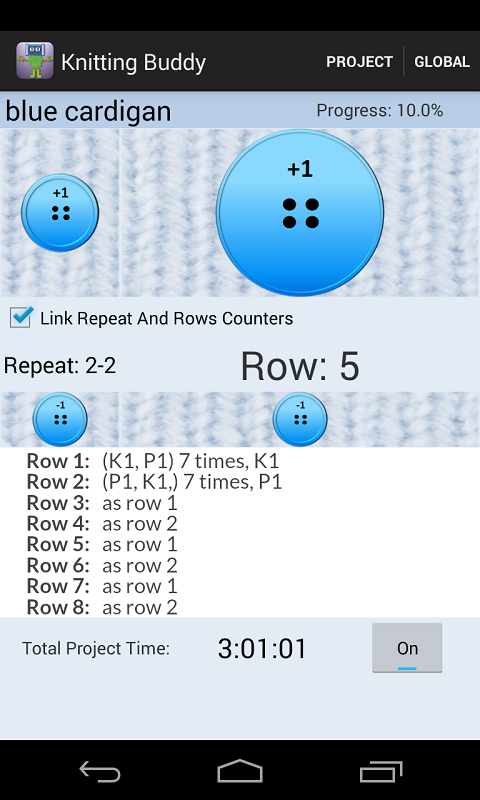
\includegraphics[width=0.95\linewidth]{images/image05.png}
        \caption[Row counter with written pattern instructions \protect{\small at: \url{https://lh3.ggpht.com/EPs72ilPpGCF_fMckHsVb2LeYVx-p6eNjcqg69eOwlsS2h0neneeMEpH29CYH3rEM_c_=h900-rw} (last accessed: 2016-04-04)}]{Row counter with written pattern instructions}
    \end{subfigure}
  \caption[Screenshots of the app Knitting and Crochet Buddy \protect{\small at: \url{https://play.google.com/store/apps/details?id=androiddeveloperjoe.knittingbuddy} (last accessed: 2016-08-08)}]{Screenshots of the app Knitting and Crochet Buddy}
\end{figure}

\addcontentsline{toc}{subsubsection}{BeeCount knitting Counter by knirirr}
\subsubsection*{BeeCount knitting Counter by knirirr}

\textit{ The app can be found at \url{https://play.google.com/store/apps/details?id=com.knirirr.beecount} \small{(last accessed: 2016-08-11)}}
\vspace*{0.5cm}

\noindent BeeCount differs from the standard of one row counter per project in that it allows multiple counters. These counters can be for parts of the knit piece that  belong to the same project, as is the case, e.g. a knitted sweater. These counters within a project can be linked together, so that increases or decreases in one counter affect the row number of another counter (see \reffigure{fig:row_counters_setup}). Furthermore, alerts can be set on different counters to be triggered once the counter
reaches a set number.

\begin{figure}[H]
  \centering
    \begin{subfigure}[b]{0.4\textwidth}
      \centering
        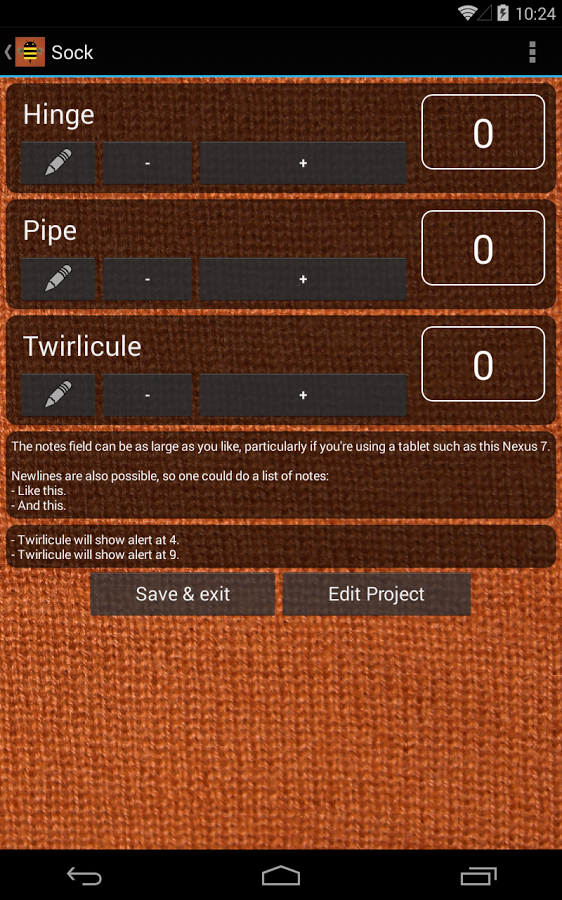
\includegraphics[width=0.95\linewidth]{images/image01.png}
        \caption[Row counters \protect{\small from: \protect\cite{beecounter_row_counters}}]{Row counters from: \protect\cite{beecounter_row_counters}}
    \end{subfigure}
    \begin{subfigure}[b]{0.4\textwidth}
      \centering
        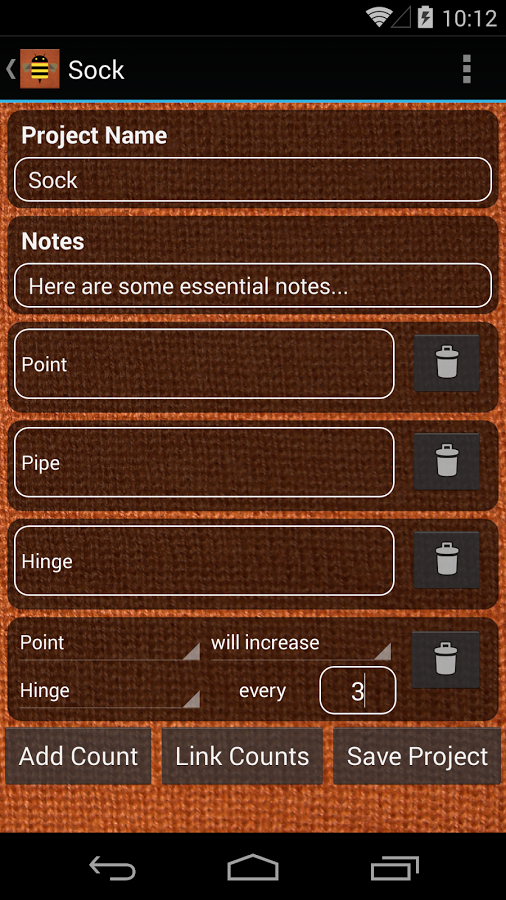
\includegraphics[width=0.95\linewidth]{images/image07.png}
        \caption[Row counters setup \protect{\small from: \url{https://lh4.ggpht.com/ZD3ujRmMgBuxEaDjnCsc9fcN9k_kUQYwfEr_mQ23n7t-0sg-arQ0MMC-I52MI7ujc94=h900-rw} (last accessed: 2016-04-04)}]{Row counters setup}
      \label{fig:row_counters_setup}
    \end{subfigure}
  \caption[Screenshots of the app BeeCount Knitting Counter \protect{\small at: \url{https://play.google.com/store/apps/details?id=com.knirirr.beecount} (last accessed: 2016-08-08)}]{Screenshots of the app BeeCount Knitting Counter}
\end{figure}

\addcontentsline{toc}{subsubsection}{Knitting Chart Maker by Awesome Applications}
\subsubsection*{Knitting Chart Maker by Awesome Applications}

\textit{The app can be found at \url{https://play.google.com/store/apps/details?id=knitting.chart.maker} \small{(last accessed: 2016-08-11)}}
\vspace*{0.5cm}

\noindent When it comes to pattern charts, none of the aforementioned apps offer a solution to input a knitting pattern chart. Only one app, the \textit{Knitting and Crochet Buddy}, has the option to include a picture of a pattern. Exception to this is the app Knitting Chart Maker, an app that focuses solely on the creation and editing of charts.

The app has over 30 stitch symbols that the user can use to create a pattern chart. The symbols are defined by the app and are not taken from a standard. The user cannot devise their own stitch symbols. Symbols can be used by selecting the symbol in the left-hand menu and then transferred onto the grid by tapping on a cell. Alternatively, the user can select the paintbrush button on the top-left menu and use their finger to paint the symbols onto every cell touched in a swiping motion, not unlike drawing with a pencil. The whole grid is zoomable up to a certain level.

While in-app, the user can purchase the pro version which allows them to save and export patterns. Charts can be exported in the form of written instructions or a picture. Included are also various sharing features, such as uploading the saved chart to Dropbox, or sharing a chart with a friend, who can then open that chart in their paid copy of the app.

The app is locked in landscape mode and the chart dimensions are limited to 50 x 50. The pattern chart grid is implemented using OpenGl’s canvas. Symbols are drawn onto the canvas via OpenGl's drawing methods for images.

\begin{figure}[H]
  \begin{center}
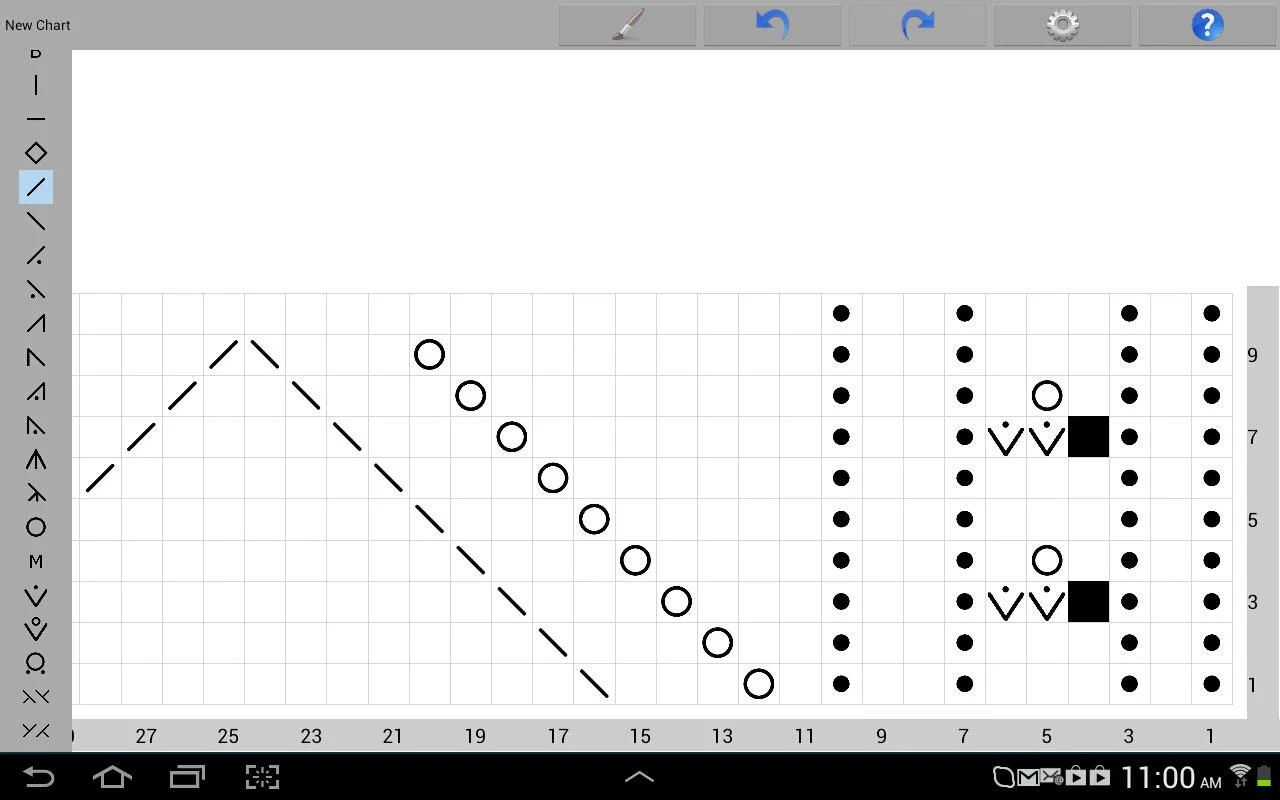
\includegraphics[width=0.7\textwidth]{images/image03.png}
\caption[Chart editor of Knitting Chart Maker \protect{\small at: \url{https://lh6.ggpht.com/MGKM0ukCDlMWWuboyxmZT-y8P3fTha4SI6l7u31eK3jFIkLsALlNEA_g6NffaoKRqyg=h900-rw} (last accessed: 2016-04-04)}]{Chart editor of Knitting Chart Maker}
\label{fig_knittingchartmaker}
\end{center}
\end{figure}

\subsection{Other}

\addcontentsline{toc}{subsubsection}{KnitML by Jonathan Whitall}
\subsubsection*{KnitML by Jonathan Whitall}

\textit{The project can be found at \url{http://www.knitml.com/blog/} \small{(last accessed: 2016-08-11)}}
\vspace*{0.5cm}

\noindent KnitML has no connection to Android, but has an honorable mentioned here since it addresses the problem of inputting a knitting pattern. KnitML is an XML based format for describing the knitting process from beginning to the finished product. The KnitML project aims to establish an international standard for knitting pattern expressions\footnote{\url{http://www.knitml.com/blog/static.php?page=about-knitml} (last accessed 2016-08-11)}. Whitall aims to do so by using the Knitting Expression Language, KEL, that he defined (\cite{knitml}). KEL is based on the Groovy programming language\footnote{\url{http://groovy-lang.org/templating.html} (last accessed 2016-08-11)} for the Java platform and the GroovyMarkup architecture.

The following KEL expression

\begin{lstlisting}[language=Java, caption=Example expression in KnitML]
Pattern {
    generalInformation
}
\end{lstlisting}

would result in

\begin{lstlisting}[language=XML, caption=Example expression in KnitML: XML result]
<pattern>
    <general-information/>
</pattern>
\end{lstlisting}

The project has not seen updates in any form since 2013 and it is presumably discontinued. A beta of an editor program for KEL and its resulting XML can be found on the homepage of the project, knitml.com.

\section{UI Evaluation}
\label{uievaluation}
As stated in the introduction (\Cref{introduction}), this thesis' goal is to produce a prototype with a useful \gls{UI}.
The term useful in this context is taken from the article \textit{Usability 101: Introduction to Usability} by \cite{nielsen2014} --- the term is used there to summarize the usability and utility of a design. Nielsen furthermore defines utility and usability as indicators of ``[...] whether [a design] provides the features you need'' and ``how easy [and] pleasant these features are to use'' (\cite{nielsen2014}).